\documentclass{standalone}
\usepackage{tikz}
\begin{document}
% Created by tikzDevice version 0.7.0 on 2015-04-30 10:54:43
% !TEX encoding = UTF-8 Unicode
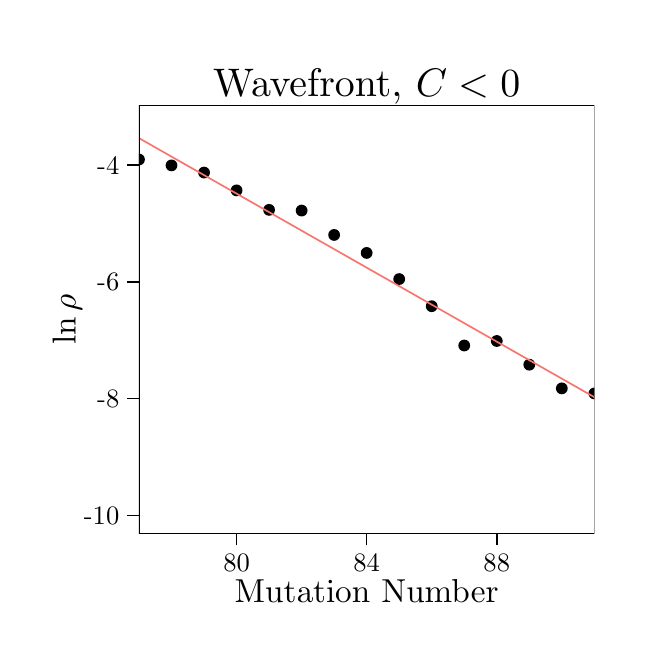
\begin{tikzpicture}[x=1pt,y=1pt]
\definecolor[named]{fillColor}{rgb}{1.00,1.00,1.00}
\path[use as bounding box,fill=fillColor,fill opacity=0.00] (0,0) rectangle (216.81,216.81);
\begin{scope}
\path[clip] (  0.00,  0.00) rectangle (216.81,216.81);
\definecolor[named]{drawColor}{rgb}{1.00,1.00,1.00}
\definecolor[named]{fillColor}{rgb}{1.00,1.00,1.00}

\path[draw=drawColor,line width= 0.6pt,line join=round,line cap=round,fill=fillColor] (  0.00,  0.00) rectangle (216.81,216.81);
\end{scope}
\begin{scope}
\path[clip] ( 40.22, 34.03) rectangle (204.76,188.82);
\definecolor[named]{fillColor}{rgb}{1.00,1.00,1.00}

\path[fill=fillColor] ( 40.22, 34.03) rectangle (204.76,188.82);
\definecolor[named]{fillColor}{rgb}{0.00,0.00,0.00}

\path[fill=fillColor] ( 40.22,169.17) circle (  2.13);

\path[fill=fillColor] ( 51.97,167.04) circle (  2.13);

\path[fill=fillColor] ( 63.73,164.45) circle (  2.13);

\path[fill=fillColor] ( 75.48,158.01) circle (  2.13);

\path[fill=fillColor] ( 87.23,150.97) circle (  2.13);

\path[fill=fillColor] ( 98.99,150.72) circle (  2.13);

\path[fill=fillColor] (110.74,141.91) circle (  2.13);

\path[fill=fillColor] (122.49,135.41) circle (  2.13);

\path[fill=fillColor] (134.25,125.97) circle (  2.13);

\path[fill=fillColor] (146.00,116.16) circle (  2.13);

\path[fill=fillColor] (157.75,101.96) circle (  2.13);

\path[fill=fillColor] (169.51,103.59) circle (  2.13);

\path[fill=fillColor] (181.26, 95.03) circle (  2.13);

\path[fill=fillColor] (193.01, 86.47) circle (  2.13);

\path[fill=fillColor] (204.76, 84.64) circle (  2.13);
\definecolor[named]{drawColor}{rgb}{0.97,0.46,0.43}
\definecolor[named]{fillColor}{rgb}{0.97,0.46,0.43}

\path[draw=drawColor,line width= 0.6pt,line join=round,fill=fillColor] ( 40.22,176.90) -- (204.76, 83.30);
\definecolor[named]{drawColor}{rgb}{0.00,0.00,0.00}

\path[draw=drawColor,line width= 0.6pt,line join=round,line cap=round] ( 40.22, 34.03) rectangle (204.76,188.82);
\end{scope}
\begin{scope}
\path[clip] (  0.00,  0.00) rectangle (216.81,216.81);
\definecolor[named]{drawColor}{rgb}{0.00,0.00,0.00}

\node[text=drawColor,anchor=base east,inner sep=0pt, outer sep=0pt, scale=  0.96] at ( 33.11, 37.25) {-10};

\node[text=drawColor,anchor=base east,inner sep=0pt, outer sep=0pt, scale=  0.96] at ( 33.11, 79.45) {-8};

\node[text=drawColor,anchor=base east,inner sep=0pt, outer sep=0pt, scale=  0.96] at ( 33.11,121.66) {-6};

\node[text=drawColor,anchor=base east,inner sep=0pt, outer sep=0pt, scale=  0.96] at ( 33.11,163.87) {-4};
\end{scope}
\begin{scope}
\path[clip] (  0.00,  0.00) rectangle (216.81,216.81);
\definecolor[named]{drawColor}{rgb}{0.00,0.00,0.00}

\path[draw=drawColor,line width= 0.6pt,line join=round] ( 35.95, 40.55) --
	( 40.22, 40.55);

\path[draw=drawColor,line width= 0.6pt,line join=round] ( 35.95, 82.76) --
	( 40.22, 82.76);

\path[draw=drawColor,line width= 0.6pt,line join=round] ( 35.95,124.97) --
	( 40.22,124.97);

\path[draw=drawColor,line width= 0.6pt,line join=round] ( 35.95,167.17) --
	( 40.22,167.17);
\end{scope}
\begin{scope}
\path[clip] (  0.00,  0.00) rectangle (216.81,216.81);
\definecolor[named]{drawColor}{rgb}{0.00,0.00,0.00}

\path[draw=drawColor,line width= 0.6pt,line join=round] ( 75.48, 29.77) --
	( 75.48, 34.03);

\path[draw=drawColor,line width= 0.6pt,line join=round] (122.49, 29.77) --
	(122.49, 34.03);

\path[draw=drawColor,line width= 0.6pt,line join=round] (169.51, 29.77) --
	(169.51, 34.03);
\end{scope}
\begin{scope}
\path[clip] (  0.00,  0.00) rectangle (216.81,216.81);
\definecolor[named]{drawColor}{rgb}{0.00,0.00,0.00}

\node[text=drawColor,anchor=base,inner sep=0pt, outer sep=0pt, scale=  0.96] at ( 75.48, 20.31) {80};

\node[text=drawColor,anchor=base,inner sep=0pt, outer sep=0pt, scale=  0.96] at (122.49, 20.31) {84};

\node[text=drawColor,anchor=base,inner sep=0pt, outer sep=0pt, scale=  0.96] at (169.51, 20.31) {88};
\end{scope}
\begin{scope}
\path[clip] (  0.00,  0.00) rectangle (216.81,216.81);
\definecolor[named]{drawColor}{rgb}{0.00,0.00,0.00}

\node[text=drawColor,anchor=base,inner sep=0pt, outer sep=0pt, scale=  1.20] at (122.49,  9.03) {Mutation Number};
\end{scope}
\begin{scope}
\path[clip] (  0.00,  0.00) rectangle (216.81,216.81);
\definecolor[named]{drawColor}{rgb}{0.00,0.00,0.00}

\node[text=drawColor,rotate= 90.00,anchor=base,inner sep=0pt, outer sep=0pt, scale=  1.20] at ( 17.30,111.43) {$\ln \rho$};
\end{scope}
\begin{scope}
\path[clip] (  0.00,  0.00) rectangle (216.81,216.81);
\definecolor[named]{drawColor}{rgb}{0.00,0.00,0.00}

\node[text=drawColor,anchor=base,inner sep=0pt, outer sep=0pt, scale=  1.44] at (122.49,191.84) {Wavefront, $C<0$};
\end{scope}
\end{tikzpicture}
\end{document}
